\section{Ambiente di calcolo distribuito}
Abbiamo un'architettura distribuita e vogliamo risolvere i problemi legati alla comunicazione sulla nostra architettura. In particolare vedremo problemi che vogliono \uline{sincronizzare i nostri processori perchè non hanno un clock globale}

\paragraph{Rappresentazione come grafo}
Un sistema distribuito è rappresentato come un grafo dove i vertici sono le entità (processori) e tra queste entità ci sono dei link (connessioni) che permettono la comunicazione tra loro. Non è detto che le connessioni siano full-duplex ma può essere anche unidirezionale.

\paragraph{Entità}
Ogni entità possiede 
\begin{itemize}
    \item Memoria locale, all'interno di questa
    \begin{itemize}
        \item Registri di input: \textbf{valore($x$)}, intendiamo l'input dell'entità $x$
        \item Registro di stato: \textbf{stato($x$)}, quello che fa capire all'entità la situazione in cui si trova. In base al proprio stato esegue certe operazioni piuttosto che altre. \uline{E' un registro che viene modificato localmente dalla stessa entità $x$}
    \end{itemize}
    \item Capacità di calcolo
    \item Capacità di comunicazione
    \item Clock locale che scandisce il tempo, non c'è una sincronizzazione tra le entità.\uline{ E' questo l'elemento che differenzia un'architettura distribuita da una parallela}.
\end{itemize}

Esempi di entità: processori, processi, sensori, switch

\paragraph{Proprietà delle entità}
\begin{enumerate}
    \item Le entità sono reattive
    
    Solo quando accade un certo \textit{evento} compiono un \textit{azione}.\\
    Un \uline{evento} può essere \uline{interno} al sistema (ricezione di messaggi, sveglia) o \uline{esterno} al sistema (impulso spontaneo/start), è l'entità che da lo start all'algoritmo distribuito
    
    Un'azione è una sequenza finita di operazioni. Cioè come rispondono i processori agli eventi. Non è possibile bloccare l'esecuzione dell'azione
    \item Le entità seguono delle regole
    \begin{definizione}
        Una regola è un oggetto della forma $stato\;x\;evento\rightarrow\;azione$
    \end{definizione}
    \begin{definizione}
        Sia $x$ un'entità, indichiamo con $B(x)$ l'insieme delle regole a cui è soggetta $x$. $B(x)$ deve essere completo e non ambiguo, cioè ad ogni evento deve essere associata un'azione e non dobbiamo associare azioni diverse allo stesso stato-evento. $B(x)$ è anche chiamato il codice di $x$, in genere vogliamo un codice che vada bene per tutte le entità

        Se $E$ è l'insieme delle entità che cooperano tra loro, $B(E) = \cup B(x)$, questo mi da l'intero comportamento del sistema. Ed è importante che sia omogeneo:
        $$\forall x,y \in E \;si\;ha\; B(x)=B(y)$$
    \end{definizione}
    \item Registro ruolo\\
    L'idea è quella di utilizzare un registro locale aggiuntivo che differenzia quelle entità che alla stessa coppia (stato, evento) hanno azioni diverse.\\
    La regola viene modificata in $\text{stato x evento} \rightarrow \text{If ruolo(x) = a then } A_a \text{ else } A_b$
\end{enumerate}

\paragraph{Proprietà della rete}
Parliamo di come le entità vedono i link. Hanno una funzione chiamata \textit{etichettatura}, la comunicazione avviene osservando le etichette
\begin{itemize}
    \item La comunicazione avviene usando una etichettatura sui link\\
    Per l'entità $x$, l'etichettatura è denotata con $\lambda x$, dato che si trova in $\vec{G}$ si indicano con
    \begin{itemize}
        \item Nin(x): vicini di ingresso di $x$
        \item Nout(x): vicini di uscita di $x$
    \end{itemize}
    \uline{Ogni entità conosce tramite la funzione $lambda$ i nomi delle porte dei link}
\end{itemize}

\paragraph{Assiomi della rete}
\begin{itemize}
        \item Ritardo finito di comunicazione. In assenza di errori, il messaggio spedito prima o poi arriverà a destinazione
        \item Orientamento locale. Ogni entità riesce a distinguere tra i suoi vicini Nin(x) e Nout(x) grazie alla conoscenza della funzione $\lambda x$
\end{itemize}

\paragraph{Parametri di rete}.\\
Numero di entità = $n$\\
Numero di link = $m$\\
Diametro della rete = $d$, è esattamente il $\delta$ delle architetture parallele 

\paragraph{Risorse di calcolo} C'è ancora il tempo, al posto dell'hardware ci sarà il costo della comunicazione quindi il numero di messaggi che definisce la congestione del sistema nel momento in cui mandiamo in esecuzione il nostro algoritmo.

Quello che è importante è sincronizzare le risorse di calcolo, non è importante che sia veloce nel computare quanto il problema venga effettivamente risolto. \uline{C'è un'atteggiamento rivolto verso la correttezza dell'algoritmo piuttosto che sul migliorare le prestazioni}. 

\paragraph{Restrizioni sulla rete}
\begin{enumerate}
    \item Restrizioni sulla comunicazione
    \begin{itemize}
        \item Link bidirezionali, assumiamo sempre che i collegamenti tra le entità siano full-duplex
        \item Ordinamento dei messaggi\\
        I messaggi sullo stesso link vengono prelevati con la politica FIFO
    \end{itemize}
    \item Restrizioni sull'affidabilità\\
    Sono in generale delle proprietà positive della rete su cui noi facciamo affidamento, quando scriviamo il codice ad esempio dichiariamo che la rete è affidabile e non ci sono errori al momento dell'esecuzione del nostro codice. 
    \begin{itemize}
        \item Affidabilità parziale, non ci saranno errori in futuro ma ci possono essere stati in passato. Può influire sulla struttura iniziale del sistema.
        \item Affidabilità totale, non ci sono stati errori in passato e non ci saranno in futuro
    \end{itemize}
    \item Restizioni sulla topologia della rete
    \begin{itemize}
        \item Connettività del grafo\\
        Ogni entità nell'ambiente distribuito possa essere raggiunta da qualsiasi altra entità. $\vec{G}$ è fortemente connesso: per ogni coppia di entità esiste un cammino che ci faccia collegare le due entità. Cammino diretto in entrambe le direzioni                                                                                                                                                                                                                                                                                                                                                                    G è connesso, comunicazione bidirezionale
    \end{itemize}
\end{enumerate}

\begin{osservazione}
Tali restrizioni a volte vengono considerate per il calcolo delle prestazioni IDEALI del codice distribuito
\end{osservazione}

\paragraph{Misure di complessità}
\begin{enumerate}
    \item Tempo distribuito\\
    L'intervallo tra la prima entità che si attiva e l'ultima che termina. \uline{Esecuzioni diverse dello stesso codice distribuito può portare a tempi diversi}. E' un problema che si risolve osservando il TEMPO IDEALE.
    \item Numero di messaggi/quantità di comunicazione
    \begin{itemize}
        \item Numero di messaggi spediti se i messaggi sono omogenei
        \item Numero di bit spediti altrimenti
    \end{itemize}
\end{enumerate}

\paragraph{Tempo ideale} 
Tempo considerando comunicazioni unitarie (un solo giro di clock), clock sincroni.

\paragraph{Tempo causale (caso peggiore)}
Tempo misurato considerando la catena più lunga di comunicazione richiesta dal codice. E' molto più difficile calcolare questo tempo perchè bisognerebbe prendere in considerazione tutte le possibili esecuzioni, perciò il più delle volte ci si rifa al tempo ideale.

\paragraph{Definizione di un problema}
Solitamente viene definito da una tripla
$$P \;=\; <P_{init},\;P_{final},\; R>$$
Dove $P_{init}$ e $P_{final}$ sono dei predicati logici che descrivono le configurazioni del sistema all'inizio e alla fine; $R$ le restrizioni del sistema

\begin{definizione}
    Definizione di configurazione: una configurazione non è altro che una fotografia (snapshot) di un sistema in un dato tempo ed è formata da
    \begin{itemize}
        \item $E(t)$ i registri delle entità al tempo $t$ per ogni $x$ del nostro ambiente
        \item Futuro(t) gli eventi già generati al tempo $t$ ma non ancora processati
    \end{itemize}
    La coppia di questi due elementi mi da la configurazione del sistema al tempo $t$
    $$C(t) = ( E(t),\;\text{Futuro}(t) )$$
\end{definizione}

\paragraph{Algoritmo distribuito: PROTOCOLLO}
Non è proprio un algoritmo inteso come sequenza di istruzioni ma abbiamo un protocollo che è considerato un \uline{insieme di regole}, in cui il programma eseguito da un'entità risulta essere un'azione causata da un certo evento. 

stato x evento $\rightarrow$ azione\footnote{Mini-programma indivisibile, cioè operazione atomica, non si può bloccare}

Il cambiamento dello stato avviene durante l'esecuzione dell'azione. Gli eventi che azionano un'entità sono: impulso spontaneo (esterno al sistema e che starta un protocollo), sveglia o ricezione di un messaggio (interni al sistema ed eseguiti durante l'esecuzione)

Un protocollo quando viene eseguito fa cambiare configurazione al sistema. \uline{L'esecuzione di un protocollo è vista come una sequenza di configurazioni successive del sistema}

\subsection{Problemi sincronizzazione/comunicazione}
\subsubsection{Broadcasting}
Risolvere il problema del broadcast significa far si che alla fine tutte le entità abbiamo la stessa
informazione
\begin{itemize}
    \item $P_{init}$: un'entità detiene I(info). Abbiamo una entità $x$ che ha l'informazione, le altre no, hanno registro valore impostato a vuoto
    \item $P_{final}$: tutte le entità posseggono I
    $$\forall x \in E \;\text{valore}(x) = I$$
    Dove $E$ è l'ambiente distribuito, vogliamo che tutte le entità abbiano la stessa informazione
    \item $R$: link bidirezionali (BL), affidabilità totale(TR, total reliability), connettività (CN), unico inziatore (UI, unique initiator)\footnote{L'impulso spontaneo che da avvio al protocollo viene fatto su una sola entità che è quella che detiene l'informazione}
\end{itemize}

\paragraph{Stati}
Utilizzeremo due stati
$$S = \{\text{iniziatore}, \text{inattivo}\}$$
$S_{init}$ stati delle entità in $C(0)$ configurazione iniziale;\\$S_{term}$ stati delle entità in $C(f)$ configurazione finale

\paragraph{Prima versione protocollo BCAST}
.\\$S_{init} = \{\text{iniziatore}, \text{inattivo}\} = S_{start}$\\
$S_{term} = \{\text{inattivo}\}$

\begin{lstlisting}
Iniziatore:
    impulso spontaneo
    {
        send (M) to N(x)
        become inattivo;
    }

Inattivo:
    ricezione(M)
    {
        processo(M);
        send(M) to N(x);
    }
\end{lstlisting}
La forma in questo caso è stato (iniziatore/inattivo) x evento (impulso spontaneo/ricezione) esegui questa azione. $N(x)$ indica i vicini.

Il messaggio M ha la seguente forma $M = (t, o, d, I)$ dove t è la tipologia del messaggio, o e d sono origine (mittente) e destinatario, I è il campo dove c'è l'informazione che deve essere prelevata e messa nei registri valore(x).

Qual'è il problema? Il protocollo è corretto ma non termina. Viene re-inviato anche il messaggio all'iniziatore (sender) che non ne ha bisogno

La risposta al problema è stabilire più stati per le nostre entità, \uline{un raffinamento degli stati $S_{term}$}. Definiamo $S_{final} \subseteq S_{term}$ come quelli stati per cui la sola azione possibile è quella nulla. \uline{Utilizziamo un nuovo stato \textit{finito} che differisce dallo stato inattivo in cui l'unica azione possibile è quella nulla}. Grazie all'uso di questo stato il protocollo riesce a terminare.

\paragraph{Seconda versione protocollo BCAST - Flooding}
.\\$S = \{\text{iniziatore}, \text{inattivo}, \text{finito}\}$\\
$S_{init} = \text{iniziatore, inattivo} = S_{start}$\\
$S_{final} = \text{finito}$

\begin{lstlisting}
Iniziatore:
    impulso spontaneo
    {
        send(M) to n(x)
        become finito
    }

Inattivo:
    ricezione(M)
    {
        processa(M);
        send(M) to n(x)-sender;
        become finito;
    }
\end{lstlisting}

\paragraph{Flooding: complessità}
Si calcola M(numero di messaggi) e T(tempo)
\begin{itemize}
    \item $M[\text{flooding}] = \sum_{x \in E} (N(x)-1) + 1 = 2m - n + 1$
    
    Dove $m$ è il numero di archi (link) ed $n$ il numero di nodi. $2m$ perchè su ogni arco viaggiano due messaggi meno quelli del sender 
    \item $T[\text{flooding} \leq d]$

    
    Dove d è il diametro della rete. Stiamo calcolando un tempo ideale, supponendo che le entità siano sincrone e che ci sia un ritardo unitario per la ricezione dei messaggi. Il tempo ideale per Flooding è d, il diametro della rete.
\end{itemize}

\paragraph{Flooding: lower bound}
Per i lower bound si ha che
\begin{itemize}
    \item $T[\text{BCAST/RI}] \geq d$
    \item $M[\text{BCAST/RI}] \geq m$
\end{itemize}
Il protocollo flooding è ottimale

\paragraph{Flooding: dimostrazione}
Teorema: $M[\text{BCAST/RI}] \geq m$

Dimostro per assurdo, risolvo il problema con meno di $m$ messaggi. Se risolvo il problema con meno di $m$ messaggi vuol dire che sul mio grafo c'è un arco su cui non viaggiano messaggi, perchè $m$ è il numero di archi sul grafo. Il protocollo risulta corretto, ma dovrebbe funzionare su tutti i G. Costruiamo un $G\prime$ per cui A non sia corretto. Otteniamo $G\prime$ da G aggiungedo un nodo non contenuto in G. Almeno un messaggio deve passare su ogni arco, altrimenti il protocollo non è corretto.

\subsubsection{Wake Up}
Nel problema BCAST avevamo un'entità che aveva l'informazione e doveva raggiungere con un messaggio tutte le altre entità. Il problema WAKE-UP si può vedere come una generalizzazione del problema BCAST dove anzichè avere una sola entità che inizia il protocollo, ne abbiamo più di una. Rilassiamo il vincolo UI(unique initiator) e facciamo si che più entità inizialmente sono attive e inviano messaggi. 

\paragraph{Protocollo WFlood}
.\\$S = \{\text{dormiente}, \text{attivo}\}$\\
$S_{init} = \{\text{dormiente}\} = S_{start}$\\
$S_{term} = \text{attivo} = S_{final}$

\begin{lstlisting}
Dormiente
    Impulso spontaneo
    {
        SEND(w) to n(x)
        become attivo
    }

    Ricezione(w)
    {
        SEND(w) to n(x)-sender
        become attivo
    }
\end{lstlisting}

Lo stato \textit{attivo} fa le veci dello stato \textit{finito} del BCAST

\paragraph{Costo}
Visto che è una generalizzazione del BCAST, possiamo considerare il tempo ideale identico a quello visto
\begin{itemize}
    \item $T[\text{WFlood}]\leq d$
    \item $2m - n + 1 \leq M[\text{WFlood}] \leq 2m$

    
    Dove $2m$ lo otteniamo se tutte le unità si svegliano con un impulso spontaneo
\end{itemize}



\subsubsection{Traversal}
Un problema che chiede ad ogni entità di essere visitata, di attivarsi sostanzialmente, attravero l'arrivo di un messaggio. Però questa visita delle entità deve avvenire sequenzialmente, cioè una alla volta. Questa è una versione ristretta di Wake-up

\paragraph{Applicazioni} Per la gestione delle risorse condivise. La risorsa è esclusiva da parte di una sola entità, per questo è utilizzata in maniera sequenziale dalle entità


\paragraph{Configurazioni}.\\
Configurazione iniziale: tutte unvisited meno una\\
Configurazione finale: tutte visited ma una alla volta

\paragraph{Protocollo Depth-first traversal}
Visita in profondità del grafo. \uline{Si scende sempre verso il vicino non ancora visitato}

Cosa facciamo quando scendiamo e visitiamo un nodo? Inviamo un messaggio che sveglia l'entità. Usiamo un messaggio particolare TOKEN T. Quando un nodo riceve T diventa visitato ma \uline{ad ogni istante di tempo viaggia al più un solo T}

\begin{enumerate}
    \item Un nodo che riceve T per la prima volta
    \begin{itemize}
        \item Ricorda il sender
        \item Fa una lista dei suoi vicini non visitati
        \item Invia T ad uno di essi
        \item Una volta inviato il token si mette in attesa. Aspetta un messaggio di ritorno da quest'ultima entità: RETURN o BACK-EDGE

        Return quando l'entità è stata svegliata per la prima volta dal token che gli è stato inviato invece \textit{Back-edge} se l'entità aveva già ricevuto il token da un'altra entità
    \end{itemize}
    \item Il vicino che riceve T
    \begin{itemize}
        \item Se è il primo T che riceve ripete 1)
        \item Altrimenti è già stato visitato e spedice un BACK-EDGE
    \end{itemize}
    \item Solo dopo aver finito la lista dei vicini non visitati deve inviare un RETURN al sender
\end{enumerate}

\paragraph{Codice}
.\\$S = \{\text{initiator}, \text{idle}, \text{visited}, \text{done}\}$\\
$S_{init} = \{\text{initiator}, \text{idle}\} = S_{start}$\\
$S_{term} = \text{done} = S_{final} $\\
Restrizioni = RI

\begin{lstlisting}
Initiator
    Spontaneously
    {
        initiator = True;
        unvisited = n(x);
        VISIT;
    }

Idle
    Receiving(T)
    {
        entry = sender;
        unvisited = n(x) - sender;
        initiator = false;
        VISIT;
    }

Visited 
    Receiving(Return)
    { VISIT; }
    
    Receiving(Back-edge)
    { VISIT; }

    Receiving(T)
    {
        unvisited = unvisited - sender;
        send(Back-edge) to sender;
    }
\end{lstlisting}

\paragraph{Procedura visit}.
\begin{lstlisting}
    if unvisited != empty then
    {
        next <- unvisited;
        send(T) to next;
        become visited;
    } else {
            if (initiator = false) then
                send (Return) to entry;
            become done;
        }
\end{lstlisting}

\paragraph{Complessità}
Se $x,y$ sono due entità su ogni link passa un messaggio token per svegliare un'entità e ci sarà una risposta (return o back-edge). Perciò su ogni link viaggiano due messaggi, non contemporaneamente. \uline{L'idea è che Traversal è sequenziale}, i messaggi viaggiano sequenzialmente.

Essendo sequenziale posso misurare il tempo ideale attraverso il numero di messaggi
$$T[\text{DF-Traversal}] = M[\text{DF-Traversal}] = 2m$$

\paragraph{Lower bound}
\begin{itemize}
    \item $M[\text{Traversal}] \geq m$ perchè vale il teorema visto per BCAST
    \item $T[\text{Traversal}] \geq n-1$ perchè ogni nodo viene visitato in sequenza
\end{itemize}

DF-Traversal è ottimo per la quantità di messaggi ma nel caso peggiore non per il tempo

\begin{osservazione}
    Il problema del costo del tempo è che ad ogni istante di tempo viaggia un messaggio solo

    Soluzione: Introduciamo concorrenza magari aggiungendo una quantità opportuna di messaggi.
\end{osservazione}

\paragraph{Problema per il protocollo} L'attesa per i \textit{back-edge} è inutile perchè perdo due unità di tempo. L'idea è questa: 

Un nodo non visitato che riceve il token comunica l'evento ai suoi vicini mandando un messaggio VISITED e lo fa in contemporanea con un token T. I vicini che ricevono VISITED aggiornano la propria lista unvisited eliminando il sender del messaggio

\paragraph{Nuova complessità}
\begin{figure}[h]
    \centering
    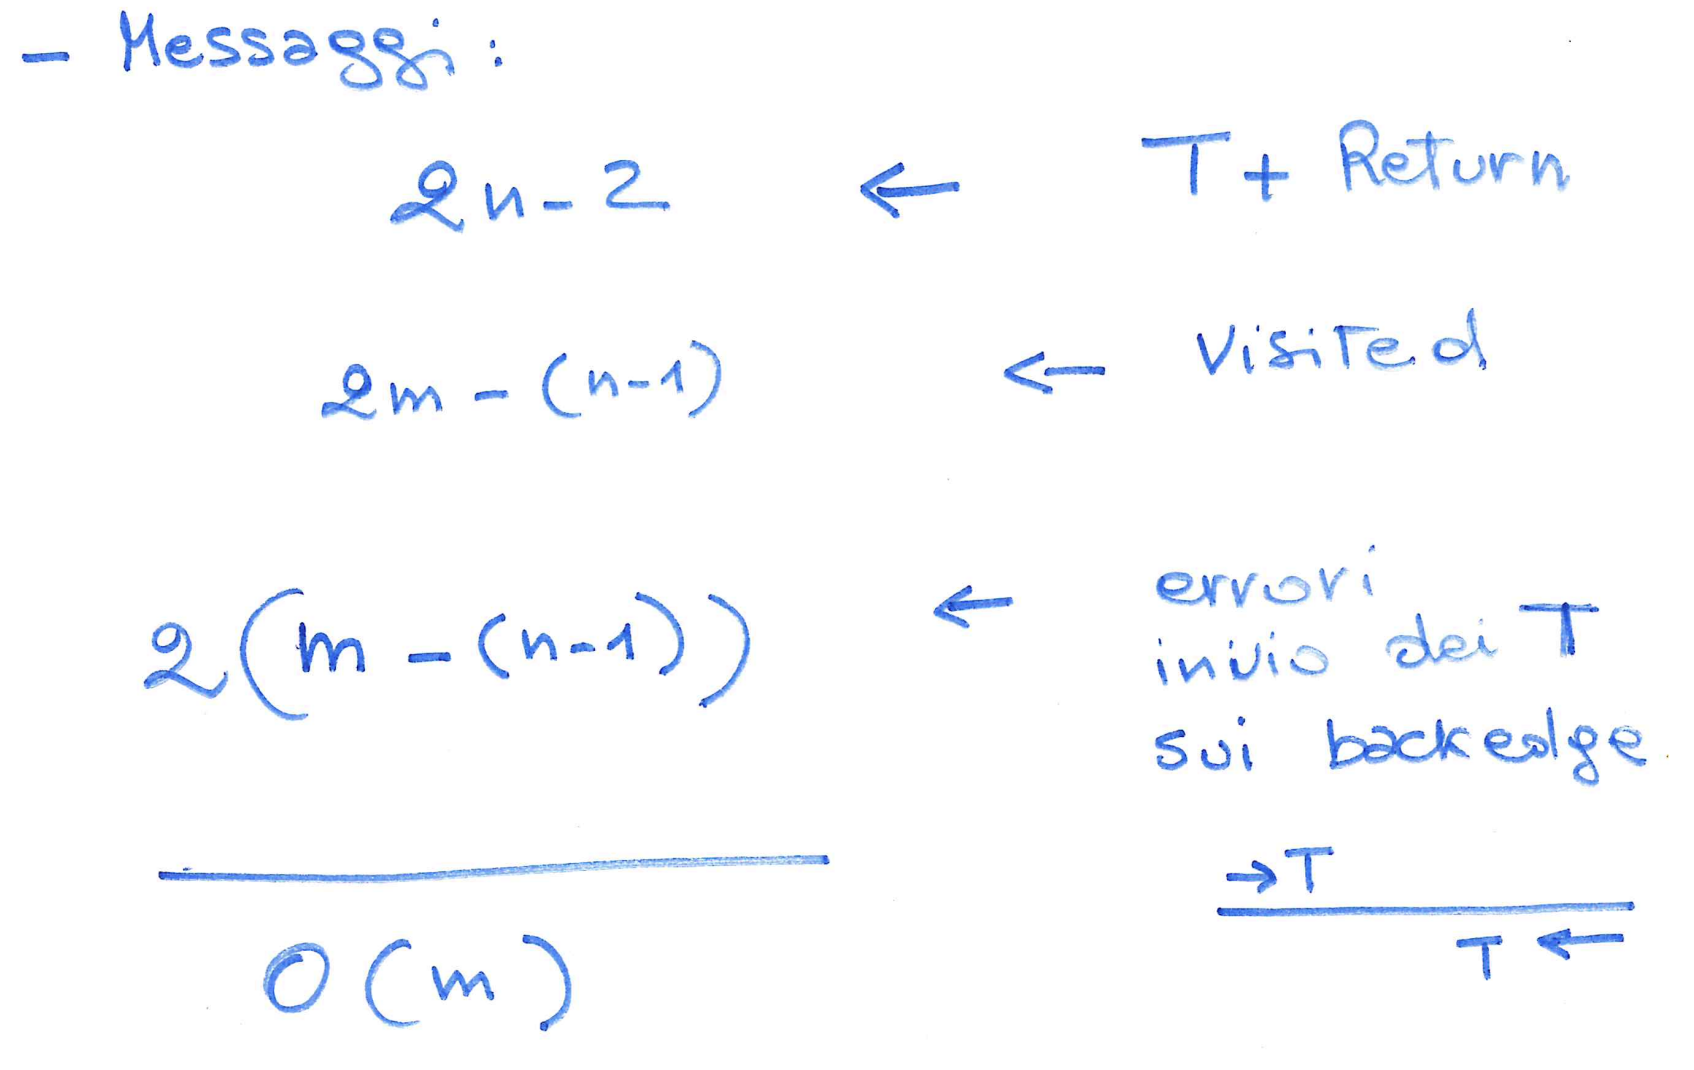
\includegraphics[scale=0.4]{images/traversal.png}
    \caption{Traversal: nuova complessità}
\end{figure}

Abbiamo aumentato il numero di messaggi però abbiamo acccelerato il protocollo.

\paragraph{Nuovo tempo}

Chiamiamo DF* il protocollo modificato con l'idea dei messaggi visited ed è ottimo per M[DF*] e T[DF*]

\subsection{Problemi rivolti all'utente finale}
\subsubsection{Spanning tree}
Costruire un'albero sulla rete dove i nodi sono un'entità di calcolo.

\begin{osservazione}
    I problemi Broadcast(BD), Wake-Up(WP), Traversal (TR) hanno una complessità di messaggi $\Theta(m)$ con 
    $$n - 1 \leq m \leq \frac{n\;(n-1)}{2} = O(n^2)$$
\end{osservazione}
dove a sinistra abbiamo l'albero, a destra il grafo completo

Lo spanning tree è importante perchè \uline{al posto di usare l'intera rete G  del grafo} (che potrebbe anche essere un grafo completo $\frac{n\;(n-1)}{2}$) \uline{usiamo una sotto-rete per minimizzare la complessità di comunicazione}, quale sottorete conviene scegliere? Quella che mi da un numero di archi $n-1$, quindi un albero

 \uline{Data una rete, costruire un albero sulla rete, così da usare l'albero per risolvere gli altri problemi}. Attenzione però ai costi per risolvere i problemi
 \begin{itemize}
     \item Costo di costruzione dell'albero
     \item Costo originale del problema eseguito su di un albero
 \end{itemize}

\paragraph{Il problema dello spanning tree}
Vogliamo costruire una sotto-rete t.c.
\begin{itemize}
    \item Coinvolge tutte le entità
    \item Le entità sono connesse
    \item E' priva di cicli
\end{itemize}

La soluzione con un algoritmo distribuito richiede la conoscenza dell'albero all'interno della rete. \uline{Ogni entità vedrà una piccola parte dell'albero}

\paragraph{Il protocollo Shout}
Shout significa 'urla, chiedi'. Ogni entità chiederà alle altre entità se esse vogliono diventare vicini nell'albero che si sta costruendo.
\begin{itemize}
    \item Ogni entità vede solo i suoi Tree\_N(x)
    \item Tiene traccia del padre
\end{itemize}

La radice dell'albero che si va a costruire è data dall'entità che inizia il protocollo (unico initiator). \uline{Si tiene traccia della radice con una variabile booleana chiamata \textit{root}, un'entità avrà root $=$ True, le altre root $=$ False}.

\begin{itemize}
    \item Iniziatore s(root) spedisce la domanda Q ai suoi vicini e attende le risposte. Chiede sostanzialmente se vogliono diventare i propri figli nell'albero
    \item Ogni entità $x \neq s$ che riceve Q
    \begin{itemize}
        \item la prima volta risponde 'yes', definendo chi è il padre cioè a chi ha inviato la risposta 'yes', ed invia Q ai suoi vicini e si mette in attesa
        \item una volta successiva alla prima risponde 'no'
    \end{itemize}
    \item Inoltre serve memorizzare l'entità padre e le entità che rispondono 'yes'
    \item L'entità termina quando riceve tutte le risposte. Bisognerà tenere traccia di quante risposte riceve, se il numero di messaggi $\text{yes}+\text{no} = Q$ può terminare
\end{itemize}

\uline{Il protocollo Shout è sostanzialmente Flooding + Reply}, perchè si fa una diffusione del messaggio Q nella rete e al messaggio Q bisogna rispondere con un 'yes' oppure un 'no'

\begin{figure}[h]
    \centering
    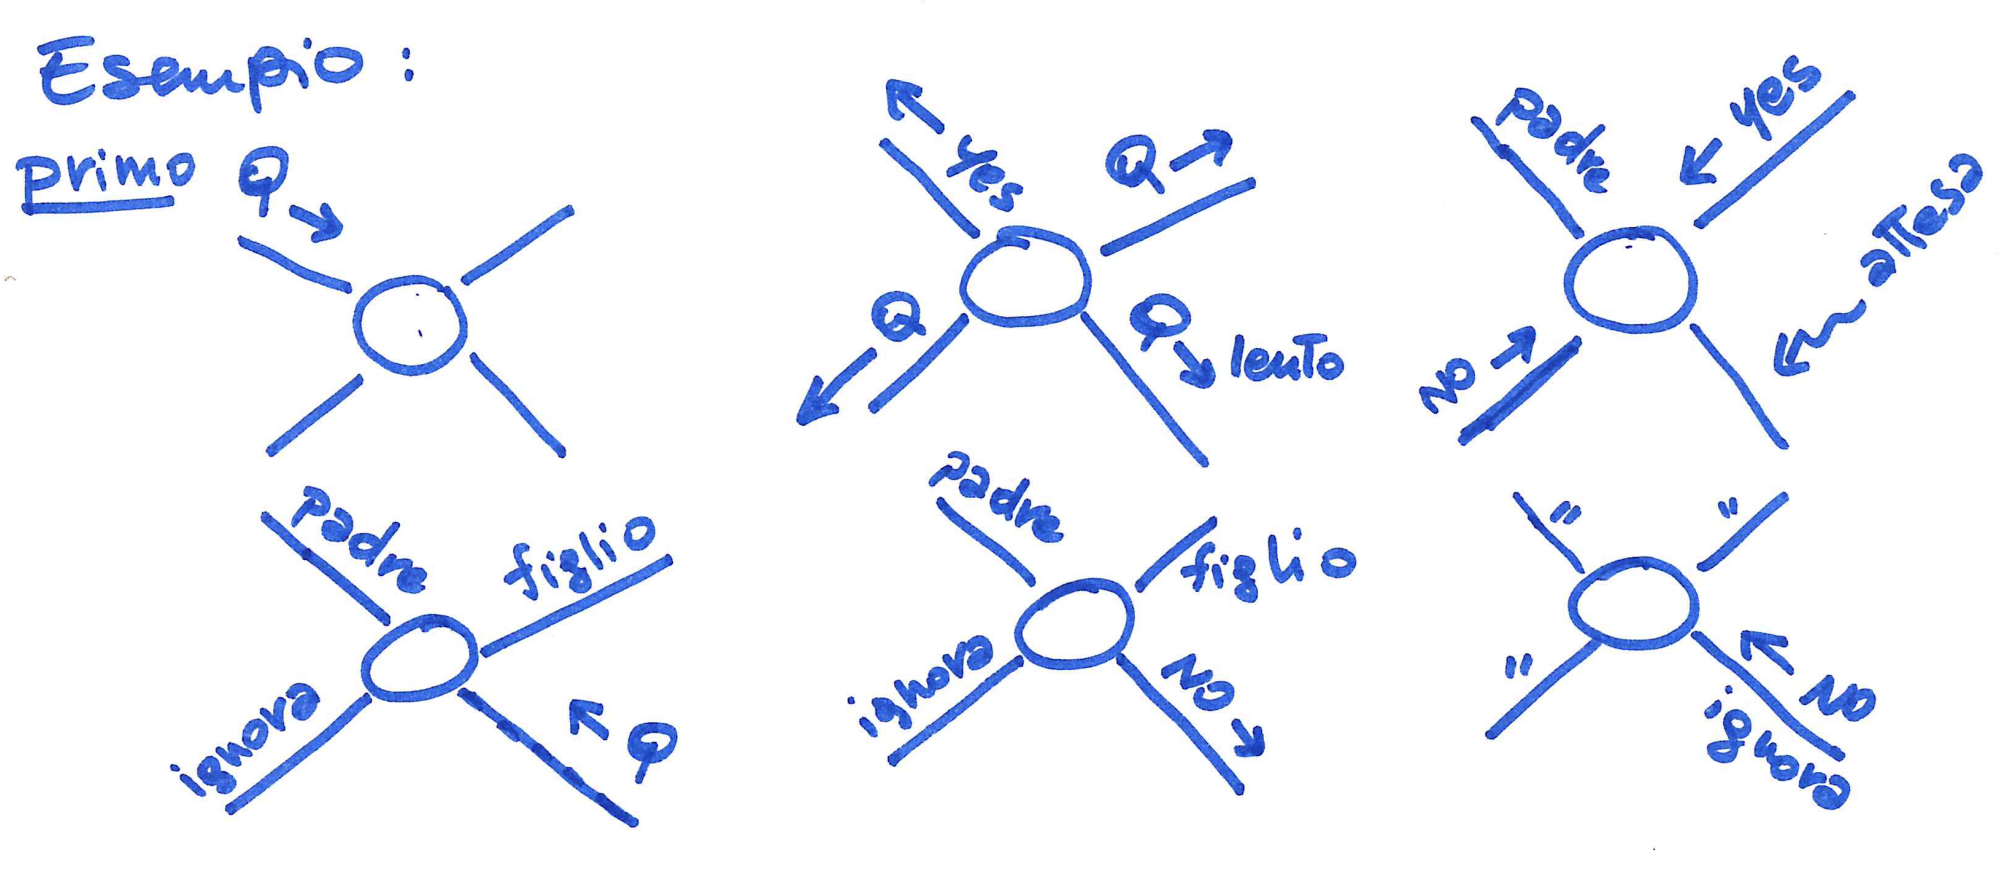
\includegraphics[scale=0.4]{images/protocollo_shout.png}
    \caption{Shout: Flooding + Reply}
    \label{fig:my_label}
\end{figure}

\paragraph{Linee guida per definire il codice}
\begin{itemize}
    \item Mandare i messaggi: Q(question), yes, no
    \item Ogni entità ha la visibilità locale dell'albero. Aggiornare variabili locali: root, parent, Tree\_n(x)\footnote{Vicini di albero: padre, figlio}, counter\footnote{Contatore che conta il numero di risposte ricevute per Q e che gli permette di terminare correttamente}
    \item Aggiornare lo stato, per raggiungere la terminazione
\end{itemize}

\paragraph{Codice}
.\\$Stati = \{\text{iniziatore}, \text{inattivi}, \text{attivi}, \text{finito}\}$\\
$S_{init} = \{\text{iniziatore}, \text{inattivi}\}$\\
$S_{final} = \text{finito}$

\begin{lstlisting}
Iniziatore
    impulso spontaneo
    {
        root = True 
        counter = 0
        tree_N(x) = empty
        send(Q) to N(x);
        become attivo;
    }
    
Inattivo
    ricezione(Q)
    {
        root = false;
        parent = sender;
        counter = 1;
        tree_N(x) = {sender};
        send('yes') sender;
        if counter = |N(x)| then
            become finito;
        else {
            send(Q) to N(x)\sender;
            become attivo;
        }
    }

Attivo
    ricezione(Q)
    { send('no') to sender }
    
    ricezione('yes')
    {
        Tree_N(x) = Tree_N(x).union{sender};
        counter = counter + 1;
        if(counter = |N(x)|) then //ha finito di ricevere le risposte
            become finito;
    }

    ricezione('no')
    {
        counter = counter + 1;
        if(counter = |N(x)|) then
            become finito;
    }
\end{lstlisting}
Solo l'iniziatore ha root True perchè abbiamo una sola radice. L'iniziatore non ha \textit{parent} perchè radice non ha padre.

Quando si riceve un 'no' praticamente il vicino non vuole essere il figlio dell'entità x, quindi non si aggiorna Tree\_N(x)
   
Nello stato finito l'unica azione che si può eseguire è quella nulla, ci si aspetta che quando tutte le entità siano in stato finito l'albero sia già stato costruito

\paragraph{Correttezza}
\begin{itemize}
    \item Terminazione: in assenza di errori riceve un numero di risposte pari ai Q inviati (le entità che seguono il protocollo Shout sono obbligate a rispondere), diventando finito
    \item Tutte le entità sono presenti/coinvolte, grazie al flooding di Q. Tutte le entità ricevono almeno un Q e vengono svegliate
    \item Le entità sono connesse
    \item E' priva di cicli: perchè ogni entità risponde con un solo 'yes' tranne la radice che risponde sempre 'no'. \uline{Per creare un ciclo si deve rispondere 'yes' almeno a due Q}
\end{itemize}

\paragraph{Costi}
Numero di messaggi
$$M[\text{Shout}] = 2M[\text{Flooding}] = 2[2n - (n-1)] = \;\approx 4m$$

Perchè su ogni link viaggia eventualmente un Q in una direzione e un Q in un'altra direzione e poi le risposte 'yes' o 'no' in una direzione e in un'altra direzione, perciò $4$ volte \textit{m}

\paragraph{Tempo}
$$T[\text{Shout}] = T[\text{Flooding}] + 1 \leq d + 1$$

E' essezialmente il tempo di diffusione del Q. Il tempo del Flooding è il diametro

\paragraph{Lower bound}
m per i messaggi, d per il tempo. Quindi abbiamo un protocollo ottimale perchè è $O(m)$ e come tempo $d+1$

\paragraph{Shout migliorato: Shout+}
Possiamo migliorare il protocollo Shout? Posso eliminare dei messaggi? Ci si chiede se questo $4m$ può essere abbassato

I messaggi che eliminiamo sono i messaggi di risposta.\\
'yes' sono necessari e si tengono, 'no' sono superflui e si possono eliminare

Questo perchè quando un'entità riceve un 'no' vuol dire che il rispondente è stato già attivato da un altro nodo e avrà già fatto il Floooding del proprio Q. \uline{L'entità $x$ attiva fa Flooding e può interpretare una risposta Q come un 'no'}

Se la risposta è un 'no' è perchè l'entità ha già ricevuto in precedenza un Q a cui ha risposto 'yes' inviando contestualmente altri Q $\implies$ se ricevo un Q lo interpreto come un 'no'

\paragraph{Nuovo costo di comunicazione Shout+}.\\
$M[\text{Shout+}] = 2m$, due messaggi soli su link


%Election
\subsubsection{Election}

\paragraph{Scopo} \uline{Stabilire un leader tra le entità di calcolo}. Individuare un'entità specifica tra tante entità autonome e omogenee (peer). Tale entità sarà chiamata \textit{LEADER} e le altre \textit{FOLLOWER}

\paragraph{Risultato di impossibilità}
E' impossibile deterministicamente individuare un leader sotto le restrizioni R (BL, CN, TR) se tutte le unità sono nello stesso stato e hanno i registri allo stesso modo

\paragraph{Risultato di possibilità}
Sotto le restrizioni RI, la starting entity\footnote{Sa di essere la starting entity perchè riceve l'impulso esterno} diventa immediatamente leader, \uline{il problema però è risolto dall'esterno e non dal sistema}. Chi stabilisce qual'è l'entità leader? Non lo stabiliscono le entità ma un evento esterno al sistema. Togliere la restrizione UI: unique initiator e ne metteremo un'altra

\paragraph{Nuova restrizione: Initial Distinct Values (ID)}
\uline{Ogni entità ha un proprio nome}. A questo punto le entità non sono più omogenee perchè hanno un elemento che le distingue che è il nome. \uline{Questo nome potrebbe anche essere un numero} 

Notazione: $R \cup \{ID\} = IR$

Sotto restrizioni IR il problema dell'election è risolvibile.

\paragraph{Strategie di soluzione}
\begin{itemize}
    \item [a)] Elect Minimum
    \begin{enumerate}
        \item Trova $id(x)$ minimo e fai $x$ leader
        \item $\forall y \neq x \in E$, y diventa follower
    \end{enumerate}
    \item [b)] Elect Minimum Initiator
    \begin{enumerate}
        \item Trova $id(x)$ minimo tra le sole entità initiator (non c'è la restrizione unique initiator) ed eleggi $x$ leader
        \item $\forall y \neq x \in E$, y diventa follower
    \end{enumerate}
\end{itemize}

\paragraph{Elect Minimum Ring}
Le mie entità sono collegate ad anello. Ogni entità ha due vicini, sinistra e destra. Siccome hanno solo due vicini, quando ricevono il messaggio arriva da uno di loro e l'altro vicino lo chiamiamo \textit{OTHER}

\paragraph{a) Protocollo All The Way}
I messaggi viaggiano intorno all'anello inoltrati dalle entità nella stessa direzione.

Tipo di messaggio sigla, mittente/entità che l'ha generato: ('Election', id(x))

Il messaggio $E$ generato da $y$ fa il giro dell'anello. Questi messaggi che girano sull'anello portano a conoscenza di tutti i nodi i nomi degli altri nodi, in questo modo tutti possono calcolare il minimo. \uline{Ogni entità riesce a collezionare gli id di tutte le entità così da calcolare il minimo}. Tutti riceveranno gli id di tutti

Quando far terminare un'entità? Una volta che $x$ riceve un messaggio con il proprio $id(x)$ sa che il messaggio ha fatto il giro dell'anello, a questo punto non lo inoltra più. Può terminare?
\begin{itemize}
    \item Solo se na ha viste $n$ diversi, se si suppone che le entità siano a conoscenza della dimensione di A ma in questo caso non c'è questa restrizione. Lavoriamo sulle restrizioni IR più il fatto che le entità sono a conoscenza di essere in un anello
    \item \uline{La risposta corretta è no}. Dobbiamo riempire in maniera oppurtuna i messaggi E ('Election', id(x), ... ) per fare terminare correttamente le entità. Aggiungiamo un contatore, il messaggio ha la seguente forma
    \[E = (\text{"Elect."}\;, id(x), \;\text{counter})\]
    \begin{itemize}
        \item Inizialmente l'entità x pone counter = 1
        \item Ogni altra entità $y \neq x$ che inoltra E somma $1$ a counter
        \item Quando E ritorna all'entità $x$ counter è uguale a $n = |A|$, in questo modo riesce a scoprire anche quant'è la dimensione di A
        \item se $x$ ha già ricevuto $n$ diversi id può terminare, altrimenti si mette in attesa
    \end{itemize}
\end{itemize}

\paragraph{Codice}
.\\$Stati = \{\text{Asleep}, \text{awake}, \text{leader}, \text{follower}\}$\\
$S_{init} = \{\text{Asleep}\}$\\
$S_{final} = \{\text{leader}, \text{follower}\}$

\begin{lstlisting}
Asleep
    spontaneously
    {
        INITIALIZE;
        become awake;
    }

    receiving('Elect', value, counter)
    {
        INITIALIZE;
        send('Elect', value, counter + 1) to OTHER
        min = Min{min, value}
        count = count + 1; 
        became awake;
    }

Awake
    receiving('Elect', value, counter)
    {
        if value != id(x) then
        {
            send('Elect', value, counter + 1) to OTHER
            min = Min{min, value}
            count = count + 1; 
            if know = True then CHECK;
            
        } else {
            size = counter;
            know = True;
            CHECK;
        }
    }
\end{lstlisting}

C'è il \textit{counter} nei messaggi che ogni entità deve incrementare e c'è il \textit{count} locale all'interno di ogni entità dove si tiene conto di quanti messaggi diversi ha visto fino a quel momento

\paragraph{Procedure INITIALIZE}
Una procedure in cui si genera il proprio messaggio
\begin{lstlisting}
    count = 0;
    size = 1;
    know = false;
    send('Elect', id(x), size) to right;
    min = id(x);
\end{lstlisting}

\textit{know} diventa True se l'entità riceve il proprio messaggio e viene a scoprire la cardinalità dell'anello

\paragraph{Procedure CHECK} 
E' una procedura che ci permette di controllare se l'entità deve terminare oppure no. Viene invocata quando è conosciuta la dimensione dell'anello.
\begin{lstlisting}
    if count = size then 
        if min = id(x) then
        { become leader; } 
        else { become follower; }
\end{lstlisting}

\paragraph{Complessità}
Numero di messaggi: $M[\text{All the way / IR} \cup \text{Ring}] = n^2$

Troppo costoso, passiamo alla strategia b)

\paragraph{b) Elect Minimum Initiator} 
Solo gli initiator generano E, mentre le altre entità inoltrano il messaggio. Facciamo l'elezione tra le sole entità che startano il protocollo. \uline{Trova l'id minimo tra le sole entità initiator}

\paragraph{Problema di terminazione}
Sebbene ogni entità che ha generato il proprio E facendo girare il messaggio riesce a scoprire il numero $n$ dell'anello, perchè ogni entità che inoltra il messaggio fa counter + 1, \uline{quelle che non hanno generato il proprio messaggio non riescono a scoprire quante entità ci sono nell'anello}. 

La conoscenza è solo delle entità initiator. Sono gli initiator che quando hanno finito e capito chi è il leader possono avvisare le altre entità. In particolare, viene fatto proprio dal leader stesso.

\paragraph{Complessità}
\begin{itemize}
    \item Numero di messaggi\\
    $M[\text{All the way - MinInitiator}] = n * k + n$ dove $k$ è il numero di initiator
    \item Tempo\\
    $M[\text{All the way - MinInitiator}] \leq 3n - 1$ considerando il caso peggiore. 
\end{itemize}

\subsubsection{Shortest Path}
Sempre un problema di comunicazione, cioè due entità che si vogliono inviare messaggi. Ma in questo caso attraverso il cammino migliore\footnote{Il cammino migliore è il cammino più corto in un grafo non pesato, o il cammino di costo minimo in un grafo pesato dove i pesi degli archi rappresentano il costo di attraversamento del messaggio su quell'arco. Questo è preferito perchè appunto abbassa i costi di comunicazione}.

\uline{Devo avere informazioni su tutti i costi della rete}. Richiede l'uso della memoria per registrare informazioni sui costi di $\vec{G}$ per ogni entità $x \in E$ al fine di calcolare i cammini minimi verso ogni altra entità, non solo verso $y$. Risolvendo il problema di comunicazione tra $x,y$ lo facciamo anche $\forall z \neq y$

\paragraph{Restrizioni}
Risolviamo il problema sotto restrizioni IR, quindi classica R + identification number. $\forall x \in E$ abbiamo id(x)

\paragraph{Full Routing Table}
Ogni strategia ha bisogno di questa tabella per risolvere il problema

\paragraph{Protocollo 1: GOSSIPING}
Richiede parecchia memoria.
Prima di costruirsi la Full Routing Table ha bisogno degli id delle entità per poterli scrivere nella colonna \textit{destinazione}

Allora si costruisce \textit{MAP(G)} che altro non è che una matrice di adiacenza\footnote{Un modo di rappresentare il grafo sotto forma tabellare} del grafo. \uline{Alla cella $(i,j)$ abbiamo il peso dell'arco tra i e j}. Abbiamo tutte le entità  sulle righe e sulle colonne e agli incroci i costi tra uno e l'altro. E' una matrice simmetrica rispetto alla diagonale.

In questo protocollo ogni entità vuole costruire questa mappa, che potrebbe essere anche molto grande. Per costruire MAP(G) in un ambiente distribuito è sufficiente che ogni entità $x$ diffonda le proprie informazioni sui vicini ad ogni altra entità $y \in E$ (fare un BROADCAST). Fare un BCAST su tutta la rete è molto costoso, in più dovrebbero farlo tutte le entità. Perciò si potrebbe costruire un albero

\paragraph{MAP-GOSSIP}
\begin{itemize}
    \item Costruzione di un albero T per G
    \item Ogni entità acquisisce dai vicini id ed i costi dei link
    \item Ogni entità diffonde le sue informazioni a tutte le altre entità usando i link di T
\end{itemize}
Una volta costruito MAP(G) ci sono tanti modi per calcolare shortest-path, ad esempio Djkstra

\paragraph{Complessità di MAP-GOSSIP}
\begin{itemize}
    \item Numero di messaggi
    \begin{itemize}
        \item Costruzione spanning tree $O(m + n \log n)$, il migliore
        \item Acquisizione informazioni dei vicini $2m$
        \item Broadcast delle informazioni $2m - 1$
    \end{itemize}
    $$M[\text{Map-Gossip}] \approx 2m * n \approx O(n^2)$$
    Quando $G$ è sparso
    \item Tempo, difficile da calcolare
\end{itemize}

Perchè Map-gossip viene scartato? Perchè non è detto che tutte le entità abbiano abbastanza memoria per mantenere una mappa del grafo, soprattutto se l'ambiente distribuito è molto grande

\paragraph{Protocollo 2: Iterated-Construction}
\uline{Richiede meno memoria} a scapito della congestione dei messaggi spediti. Aumenta anche il tempo

La Full Routing Table viene costruita a più riprese. \uline{Si evita di costruire la MAP(G)} e si va direttamente a costruire la tabella attraverso un processo di iterazioni in cui c'è uno scambio di messaggi tra le entità. \uline{Ogni entità si costruisce la sua Full Routing Table senza utilizzare MAP(G), così evitiamo lo spreco di memoria}. Inizialmente la F.R.T. contiene solo informazioni dei vicini, con costo $\infty$ per i non vicini che verrà sostiuito alle iterazioni successive con un valore più ragionevole

\begin{osservazione}
    Se vogliamo una Routing Table più corta, è possibile che al posto dello \textit{shortest path} ci mettiamo il vicino coinvolto nel cammino. Con questo riusciamo a ridurre la quantità di memoria necessaria
\end{osservazione}

\paragraph{Distance Vector}
Ogni entità si costruisce una F.R.T parziale e ad ogni iterazione questa tabella viene aggiornata, ad ogni iterazione si spedisce ai vicini delle informazioni. Queste informazioni vengono ricevute dalle entità che aggiorna la propria F.R.T. Le informazioni che si spediscono sono il Distance Vector

Sulla base delle informazioni che gli arrivano dai vicini stabilisce se sono stati trovati cammini minimi migliori di quelli che ha nella propria FRT e in tal caso aggiorna la FRT

\paragraph{Notazione} $V_x[z]$ è il costo del cammino minimo da $x$ a $z$

\begin{definizione}
    E' la F.R.T. ristretta alle colonne Destination e Cost e viene indicata con V
\end{definizione}

\paragraph{Numero di iterazioni} $n-1$, si può dimostrare per induzione

\paragraph{Complessità Iterated-Construction}
E' un protocollo con più iterazioni. Il numero di iterazioni è $n-1$
\begin{itemize}
    \item Numero di messaggi
    $$M[\text{ItConstr / IR}] = 2m * n * (n-1)$$
    Su ogni arco abbiamo due spedizioni di Distance Vector che costano $n$, ripetuta per $n-1$ iterazioni
    \item Tempo
    $$M[\text{ItConstr / IR}] = (n-1) * \tau(n)$$
    Ci sono sempre $n-1$ iterazioni dove in ogni iterazioni vengono spediti le V (Distance Vector). $\tau(n)$ è il tempo ideale per trasmettere una V. 
\end{itemize}



